\chapter{Conjuntos, Funções, Matrizes e Sequências}%sequencias e matrizes no
% futuro
\label{cap:conjuntos}

\section{Conjuntos}

\subsection*{\underline{Introdução}}

Nesta secção estudaremos as estruturas discretas fundamentais nas quais todas as
outras estruturas discretas são construídas, nomeadamente, os conjuntos. Os
conjuntos são utilizados para agrupar objectos. Geralmente, mas não sempre, os
objectos num conjunto possuem propriedades semelhantes. Por exemplo, todos os
estudantes que estão inscritos na Universidade Agostinho Neto formam um
conjunto. Da mesma forma, todos os estudantes actualmente inscritos na
disciplina de Estruturas Discretas em qualquer Universidade formam um conjunto. Além disso, estes
estudantes inscritos na Universidade Agostinho Neto e inscritos na disciplina de
Estruturas Discretas formam um conjunto composto pelos os elementos em comum
das duas primeiras coleções.

A linguagem dos conjuntos é uma forma de se estudar tais coleções de forma
organizada. Daremos a seguir uma definição do termo ``conjunto''. Esta definição
é apenas intuitiva e não é parte da definição formal da teoria dos conjuntos.

\label{def31}
\begin{defn}
(Conjunto) Um conjunto é uma colecção não-ordenada de objectos, chamados de
\emph{elementos} ou \emph{membros} do conjunto. Diz-se que um conjunto
\emph{contém} elementos. Escrevemos $a \in A$ para denotar que $a$ é um
elemento do conjunto. A notação $a \notin A$ denota que $a$ não é um elemento
do conjunto $A$.
\end{defn}

É comum representar os conjuntos com letras maiúsculas. As letras minúsculas são
geralmente utilizadas para denotar os elementos dos conjuntos. Existem diversas
formas de descrever um conjunto. Uma delas é por listar todos os elementos do
conjunto, quando isto é possível. Utilizamos as chavetas para denotar um
conjunto com todos os elementos listados. Por exemplo, a notação $\{a,b,c,d\}$
representa o conjunto com os quatro elementos $a,b,c$ e $d$. Esta forma de
descrever um conjunto é conhecida como \textbf{método de listagem}.

\label{exem31}
\begin{exmp}
O conjunto $V$ de todas as vogais no alfabeto Português pode ser escrito como $V
= \{a,e,i,o,u\}$.
\end{exmp}
\label{exem32}
\begin{exmp}
O conjunto I de todos os inteiros positivos menores que 10 pode ser escrito como
$I=\{1,3,5,7,9\}$.
\end{exmp}
\label{exem33}
\begin{exmp}
Embora os conjuntos são geralmente utilizados para agrupar elementos com
propriedades comuns, não existe alguma restrição que impeça-os de possuírem
elementos não relacionados. Por exemplo, $\{a, 2,$ Francisco$,$ Malange$\}$ é o
conjunto que contêm os quatro elementos $a, 2,$ Francisco e Malanje.
\end{exmp}

Por vezes o método de listagem é utilizado para descrever um conjunto sem listar
todos os seus elementos. Alguns elementos são listados e a seguir elípses ou
reticências (\ldots) são acrescentadas quando o padrão geral dos elementos é
óbvio.

\label{exem34}
\begin{exmp}
O conjunto dos números positivos inteiros menores que 100 pode ser denotado por
$\{1,2,3,\ldots,99\}$.
\end{exmp}

Uma outra forma de descrever um conjunto é por utilizar um \textbf{constructor
de conjunto}. Caracterizamos os elementos de um conjunto por definir uma
propriedade ou propriedades que os elementos devam possuír para fazer parte do
conjunto. Por exemplo, o conjunto $I$, de todos os números positivos inteiros
menores que $10$ pode ser escrito como:

\begin{center}$O = \{x \mid x$ é um inteiro positivo menor que 10.$\}$\end{center}

\noindent ou, especificando o universo como o conjunto dos inteiros positivos,
da seguinte maneira:

\begin{center}$O = \{x \in \mathbb{Z}^{+} \mid x$ é impar e $x < 10\}$\end{center}

Geralmente utilizamos esta notação para descrever conjuntos onde é impossível
listar todos os elementos do conjunto. Por exemplo, o conjunto $\mathbb{Q}^{+}$
de todos os números racionais positivos pode ser escrito como:

\begin{center}$\mathbb{Q}^{+} = x \in \mathbb{R} \mid x = \frac{p}{q}$ para alguns
inteiros positivos $p$ e $q$.\end{center}

Cada um dos conjuntos abaixo, denotados por uma letra maiúscula a negrito, tem
um papel importante na matemática discreta:

\begin{enumerate}
  \item  $\textbf{N} = \{0,1,2,3,\ldots\}$, o conjunto dos \textbf{números
  naturais}
  \item $\textbf{Z} = \{\ldots,-2,-1,0,1,2,\ldots\}$, o conjunto dos
  \textbf{inteiros}
  \item $\textbf{Z}^+ = \{1,2,\ldots\}$, o conjunto dos \textbf{inteiros
  positivos}
  \item $\textbf{Q} = \{p/q$ \mid $p \in \textbf{Z}, q \in \textbf{Z},$ e $ q
  \neq 0\}$, o conjunto dos \textbf{números racionais}
  \item $\textbf{R}$, o conjunto dos \textbf{números reais}
  \item $\textbf{R}^+$, o conjunto dos \textbf{números reais positivos}
  \item $\textbf{C}$, o conjunto dos \textbf{números complexos}
\end{enumerate}

Note que que algumas pessoas não consideram o $0$ como um número natural,
portanto tena cuidado na utilização do termo \emph{número natural} quando lê
outros conteúdos/livros.

Conjuntos podem ter outros conjuntos como seus elementos, como ilustra o exemplo
\ref{exem35}.


\begin{exmp}
\label{exem35}
O conjunto $\{\textbf{N,Z,Q,R}\}$ é um conjunto constituído por quatro
elementos, sendo cada um deles um conjunto.
\end{exmp}

\begin{description}
\item[\emph{Nota}:] O conceito de tipo de dados na Ciência da Computação é
construído sobre o conceito de um conjunto. Em particular um \textbf{tipo de
dados} é o nome de um conjunto, juntamente com um conjunto de operações que
podem ser realizadas nos objectos de tal conjunto. Por exemplo, \emph{boolean} é
o nome do conjunto $\{0,1\}$ juntamente com as operações em um ou mais elementos
deste conjunto, tais como AND, OR e NOT.
\end{description}

Como muitas sentenças matemáticas afirmam que duas coleções de
objectos especificadas de forma diferente são na verdade o mesmo
conjunto, precisamos entender o que significa igualdade de dois
conjuntos.

\label{def32}
\begin{defn}
Dois conjuntos são \emph{iguais} se e somente se possuem os mesmos elementos.
Portanto, se $A$ e $B$ são conjuntos, então $A$ e $B$ são iguais se e somente se
$\forall x (x \in A \leftrightarrow x \in B)$. Escrevemos $A = B$ se $A$ e $B$
são conjuntos iguais.
\end{defn}

\label{exem36}
\begin{exmp}
Os conjuntos $\{1,3,5\}$ e $\{3,5,1\}$ são iguais porque possuem os mesmos
elementos. Note que a ordem em que os elementos de um conjuntos são listados não
interessa. Note também que não importa se um elemento de um conjunto é listado
mais de uma vez, portanto, o conjunto $\{1,3,3,3,5,5,5,5\}$ é o mesmo conjunto
que $\{1,3,5\}$ pois possuem os mesmos elementos.
\end{exmp}

\begin{description}
\item[O CONJUNTO VAZIO] Existe um conjunto especial que não possui elementos.
Este conjunto é chamado de \textbf{conjunto vazio} ou \textbf{conjunto nulo}, e
é denotado por $\emptyset$. O conjunto vazio pode também ser denotado por $\{
\}$ (isto é, representamos o conjunto com um par de chavetas que inclui todos
os elementos neste grupo). Geralmente, um conjunto de elementos com certas
propriedades acaba por transformar-se num conjunto vazio. Por exemplo, o
conjunto de todos os inteiros positivos que são maiores que os seus quadradados
é um conjunto vazio.
\end{description}

Um conjunto com apenas um elemento é chamado de \textbf{conjunto unitário}. Um
erro comum é confundir o conjunto vazio $\emptyset$ com o conjunto
$\{\emptyset\}$, que é um conjunto unitário. O único elemento do conjunto
$\{\emptyset\}$ é o próprio conjunto vazio! Uma analogia útil para lembrar-se
desta diferença é pensar nos directórios ou pastas de um computador. O conjunto
vazio nesta analogia seria um pasta vazia e o conjunto composto pelo conjunto
vazio seria uma pasta com apenas um elemento, nomeadamente, uma pasta vazia.

\subsection*{\underline{Subconjuntos}}

É comum encontrarmos situações onde os elementos de um conjunto são tamb´´em os
lementos de um segundo conjunto. Iremos agora introduzir alguma terminologia e
notações para expressar estas relações entre conjuntos.

\begin{defn}
\label{def33}
O conjunto $A$ é um \emph{subconjunto} de $B$ se e somente se todo elemento de
$A$ é também um elemento de $B$. Utilizamos a notação $A \subseteq B$
para indicar que $A$ é um subconjunto do conjunto $B$.
\end{defn}

Nós vemos que $A \subseteq B$ se e somente se a quantificação
\begin{center}$\forall x (x \in A \to x \in B)$\end{center}
\noindent é verdadeira. Note que para provar que $A$ não é um subconjunto de $B$
precisamos apenas encontrar um elemento $x \in A$ com $x \notin B$. Um elemento
$x$ com estas características é chamado de contra-exemplo da afirmação de que
$x \in A$ implica $x \in B$.

\begin{exmp}
\label{exem37}
O conjunto de todos os números ímpares positivos menores que 10 é um subconjunto
do conjunto de todos os inteiros positivos menores que 10. O conjunto dos
números racionais é um subconjunto do conjunto dos números reais.
\end{exmp}

\begin{description}
\item[Teorema 1] Para todo conjunto $S$, $\emptyset \subseteq S$ e $S \subseteq
S$
\end{description}

Para mostrar que dois conjuntos são $A$ e $B$ são iguais, mostre que $A
\subseteq B$ e $B \subseteq A$. Os conjuntos podem ter outros conjuntos como
membros. Por exzemplo, temos os conjuntos
\begin{center}
$A = \{\emptyset, \{a\}, \{b\}, \{a,b\}\}$ e $B = \{x \mid x$ é um subconjunto
do conjunto $\{a,b\}\}$
\end{center}

Note que estes dois conjuntos são iguais, isto é, $A = B$. Note também que
$\{a\} \in A$, mas $a \notin A$.

\subsection*{\underline{O Tamanho de um Conjunto}}

Conjuntos são extensivamente utilizados em problemas de contagem, e para esta
utilização precisamos discutir o tamanho dos conjuntos.

\begin{defn}
\label{def34}
Seja $S$ um conjunto. Se existem exactamente $n$ elementos distintos em $S$ onde
$n$ é um inteiro não negativo, dizemos que $S$ é um \emph{conjunto finito} e que
$n$ é a cardinalidade de $S$. A cardinalidade de $S$ é denotada por $\mid
S \mid$.
\end{defn}

\begin{defn}
\label{def35}
Um conjunto é chamado de \emph{infinito} quando não é finito.
\end{defn}

\subsection*{\underline{Conjunto - Potência}}
Muitos problemas envolvem a necessidade de testar todas as combinações possíveis
de elementos de um conjunto para ver se os mesmos satisfazem alguma propriedade.
Para considerar todas estas combinações de elementos de um conjunto $S$,
construímos um novo conjunto que possui como elementos, todos os subconjuntos de
$S$.

\begin{defn}
\label{def36}
Dado um conjunto $S$, o conjunto-potência de $S$ é o conjunto de todos os
subconjuntos do conjunto $S$. O conjunto-potência de $S$ é denotado por
$\mathcal{P}$.
\end{defn}

\begin{exmp}
\label{exem38}
Qual é o conjunto-potência do conjunto $\{0,1,2\}$?

\begin{description}
\item[Solução:] O conjunto-potência $\mathcal{P}(\{0,1,2\})$ é o cojunto de
todos os subconjuntos de $\{0,1,2\}$. Sendo assim
\begin{center}
$\mathcal{P}(\{0,1,2\}) = \{\emptyset, \{0\}, \{1\}, \{2\}, \{0,1\}, \{0,2\},
\{1,2\}, \{0,1,2\}\}$.
\end{center}
\end{description}

\end{exmp}



\begin{exmp}
\label{exem39}
Qual é o conjunto-potência do conjunto vazio? Qual é o conjunto potência do
conjunto $\{\emptyset\}$?

\begin{description}
\item[Solução:]O conjunto vazio possui exactamente um subconjunto, nomeadamente,
sí próprio. Consequentemente
\begin{center}
$\mathcal{P}(\emptyset) = \{\emptyset\}$.
\end{center}
O conjunto $\{\emptyset\}$ possui exactamente dois subconjuntos, nomeadamente,
$\emptyset$ e o conjunto $\{\emptyset\}$. Portanto,
\begin{center}
$\mathcal{P}(\{\emptyset\}) = \{\emptyset, \{\emptyset\}\}$.
\end{center}
\end{description}
\end{exmp}
Se um conjunto possui $n$ elementos, então o seu conjunto-potência possui $2^n$
elementos. Iremos demonstrar este facto de várias formas em secções
subsequentes.

\subsection*{\underline{Produto Cartesiano}}

A ordem dos elementos numa coleção geralmente é importante. Como os conjuntos
são não-ordenados, uma estrutura diferente é necessária para representar
coleções ordenadas. Isto é providenciado pelas \textbf{n-tuplas ordenadas}.

\begin{defn}
\label{def37}
A \emph{n-tupla ordenada} $(a_1, a_2, \ldots, a_n)$ é a coleção ordenada que
possui $a_1$ como o seu primeiro elemento, $a_2$ como o seu segundo, \ldots, e
$a_n$ como o seu $n^o$ elemento (ou elemento de ordem n).
\end{defn} 

Dizemos que duas $n$-tuplas ordenadas são iguais se e somente se cada par
correspondente dos seus elementos são iguais. Por outras palavras, $(a_1, a_2,
\ldots,a_n) = (b_1, b_2, \ldots, b_n)$ se e somente se $a_i = b_i$, para
$i=1,2,\ldots,n$. Em particular, 2-tuplas ordenadas são chamadas de
\textbf{pares ordenados}. Os pares ordenados $(a,b)$ e $(c,d)$ são iguais se e
somente se $a = c$ e $b = d$. Note $(a, b)$  e $(b,a)$ não são iguais ao menos
que $a = b$.

Muitas das estruturas discretas que iremos estudar em capítulos posteriores são
baseadas na noção de \emph{produto Cartesiano} (em homenagem ao matemático
francês René Descartes). Iremos primeiramente definir o produto cartesianos de
dois conjuntos.

\begin{defn}
\label{def38}
Sejam $A$ e $B$ dois conjuntos. O \emph{produto Cartesiano} de $A$ e $B$,
denotado por $A \times B$, é o conjunto de todos os pares ordenados $(a, b)$,
onde $a \in A$ e $b \in B$. Assim,
\begin{center}
$A \times B = \{(a,b) \mid a \in A \land b \in B\}.$
\end{center}
\end{defn}

\begin{exmp}
\label{exem310}
Qual é o produto Cartesiano de $A = \{1,2\}$ e $B = \{a,b,c\}$?
\begin{description}
\item[Solução:]O produto Cartesiano $A \times B$ é
\begin{center}
$A \times B = \{(1,a), (1,b), (1,c), (2,a), (2,b), (2,c)\}$.
\end{center}
Note que o produto Cartesiano $A \times B$ e $B \times A$ não são equivalentes,
ao menos que $A = \emptyset$ ou $B = \emptyset$ (de tal forma que $A \times B
= \emtyset$) ou $A = B$. Isto é ilustrado no exemplo \ref{exem311}.
\end{description}
\end{exmp}

\begin{exmp}
\label{exem311}
Mostre que o produto Cartesiano $B \times A$ não é igual ao produto cartesiano
$A \times B$ onde $A$ e $B$ são os mesmos do exemplo \ref{exem310}.
\begin{description}
\item[Solução:] O produto Cartesiano $B \times A$ é
\begin{center}
$B \times A = \{(a,1), (a,2), (b,1), (b,2),(c,1),(c,2)\}$.
\end{center}
Este resultado é diferente de $A \times B$ obtido no exemplo \ref{exem310}.
\end{description}
\end{exmp}

\begin{defn}
\label{def39}
O \emph{producto Cartesiano} dos conjuntos $A_1, A_2, \ldots, A_n$, denotado por
$A_1 \times A_2 \times \ldots \times A_n$, é o conjunto de pares ordenados de
$n$-tuplas ordenadas $(a_1, a_2, \ldots,a_n)$ onde $a_i$ pertence a $A_i$ para
$i = 1,2,\ldots,n$. Em outras palavras,
\begin{center}
$A_1 \times A_2 \times \ldots \A_n = \{(a_1, a_2,\ldots,a_n) \mid a_i \in
A_i$ para $i = 1,2,\ldots,n\}$.
\end{center}
\end{defn}

\begin{exmp}
\label{exem312}
Qual é o produto Cartesiano $A \times B \times C$, onde $A = \{0,1\}, B=\{1,2\}$
e $C = \{0,1,2\}$?
\begin{description}
\item[Solução:]O produto Cartesiano $A\times B\times C$ consiste em todas as
triplas ordenadas $(a,b,c)$, onde $a \in A$, $b \in B$, e $c \in C$. Assim,
\begin{center}
$A\times B\times C =
\{(0,1,0),(0,1,1),(0,1,2),(0,2,0),(0,2,1)\\,(0,2,2),(1,1,0),(1,1,1),(1,1,2),(1,2,0),(1,2,1),(1,2,2)\}$
\end{center}
\end{description}
\end{exmp}


\subsection*{\underline{Utilizando a Notação de Conjuntos com Quantificadores}}

Por vezes restringimos o domínio de um sentença quantificada por explicitamente
utilizar uma notação em particular. Por exemplo, $\forall x\in S(P(x))$ denota a
quantificação universal de de $P(x)$ para todos os elementos do conjunto $S$. Em
outras palavras, $\forall x\in S(P(x))$ é a simplificação de $\forall x (x \in
S \to P(x))$. Similarmente, $\exists x\in S(P(x))$ denota a quantificação
existêncial de $P(x)$ sobre os elementos em $S$. Isto é, $\exists x\in S(P(x))$
é a simplificação de $\exists x(x \in S \land P(x))$.

\begin{exmp}
\label{exem313}
O que é que as sentenças $\forall x\in \textbf{R}(x^2 \geq 0)$ e $\exists x \in
\textbf{Z}(x^2 = 1)$ significam?
\begin{description}
\item[Solução:] A sentença $\forall x\in \textbf{R}(x^2 \geq 0)$ afirma que para
todos os números reais $x$, $x^2 \geq 0$. Esta sentença pode ser expressa como
``O quadrado de todo o número real é não-negativo''.

A sentença $\exists x \in \textbf{Z}(x^2 = 1)$ afirma que existe um número
inteiro $x$ tal que $x^2 = 1$. Esta sentença
pode ser expressa como ``Existe um inteiro cujo o quadrado é igual a 1''.
\end{description}
\end{exmp}

\subsection*{\underline{Conjunto-verdade e Quantificadores}}

Iremos agora alinhar os conceitos da teoria dos conjuntos e da lógica de
predicados. Dado um predicado $P$, e um domínio $D$, definimos o
\textbf{Conjunto-verdade} de $P$ como sendo o conjunto de elementos $x$ em $D$
para os quais $P(x)$ é verdade. O conjunto-verdade de $P(x)$ é denotado por
$\{x \in D \mid P(x)\}$.

\begin{exmp}
\label{exem314}
Quais são os conjuntos-verdade dos predicados $P(x), Q(x)$ e $R(x)$, onde o
domínio é o conjunto dos números inteiros e $P(x)$ é ``$|x| = 1$'', $Q(x)$ é
``$x^2 = 2$'' e $R(x)$ é ``$|x| = x$''.
\begin{description}
\item[Solução:]O conjunto-verdade de $P$, $\{x \in \textbf{Z} \mid |x| = 1\}$, é
o conjunto de inteiros para os quais $|x| = 1$. Como $|x| = 1$ quando $x=1$ ou
$x=-1$, e para mais nenhum outro inteiro $x$, vemos que o conjunto-verdade de
$P$ é o conjunto $\{-1,1\}$.

O conjunto-verdade de $Q$, $\{x \in \textbf{Z} \mid x^2 = 2\}$, é o conjunto de
inteiros para os quais $x^2 = 2$. Este conjunto é vazio porque não existe um
número inteiro $x$ para os quais $x^2 = 2$.

O conjunto-verdade de $R$, $\{x \in \textbf{Z} \mid |x| = x\}$, é o conjunto de
inteiros para os quais $|x| = x$. Como $|x| = x$ se e somente se $x \geq 0$,
acontece que o conjunto-verdade de $R$ é o conjunto $\textbf{N}$, o conjunto
dos números inteiros não-negativos.
\end{description}
\end{exmp}

\section{Operações sobre Conjuntos}

\subsection*{\underline{Introdução}}

Dois ou mais conjuntos podem ser combinados de diversas formas. Por exemplo,
começando com o conjunto das disciplinas do curso de Matemática da tua
universidade e o conjunto das disciplinas do curso de Ciência da Computação,
podemos formar o conjunto dos estudantes que têm disciplinas do curso de
Matemática e do curso de Ciência da Computação, o conjunto dos estudantes que
têm disciplinas dos dois cursos e por aí em diante.

\begin{defn}
\label{def310}
Sejam $A$ e $B$ dois conjuntos. A \emph{união} dos conjuntos $A$ e $B$, denotada
por $A \cup B$, é o conjunto que contém os elementos que estão em $A$ ou em $B$,
ou em ambos.
\end{defn}

Um elemnto $x$ pertence a união dos conjuntos $A$ e $B$ se e somente se $x$
pertence a $A$ ou $x$ pertence a $B$. Isto nos diz que
\begin{center}
$A \cup B = \{x \mid x\in A \lor x\in B\}.$
\end{center}

O diagrama de Venn (\emph{Pesquisar sobre Diagramas de Venn}) da figura
\ref{fig31} representa a união dos conjuntos $A$ e $B$. A area que representa
$A \cup B$ é a área sombreada entre os círculos que representam $A$ ou que
representam $B$.

\begin{figure}[H]
	\centering
	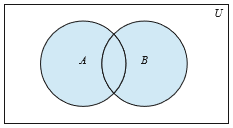
\includegraphics[scale=2]{chapter/imagens/31}
	\caption{Diagrama de Venn da união de $A$ e $B$.}
	\label{fig31}
\end{figure}

\begin{exmp}
\label{exem315}
A união dos conjuntos $\{1,3,5\}$ e $\{1,2,3\}$ é o conjunto $\{1,2,3,5\}$; isto
é, $\{1,3,5\} \cup \{1,2,3\} = \{1,2,3,5\}$.
\end{exmp}

\begin{defn}
\label{def311}
Sejam $A$ e $B$ dois conjuntos. A \emph{intersecção} dos conjuntos $A$ e $B$,
denotada por $A \cap B$, é o conjunto que contém os elementos que estão tanto em
$A$ como em $B$.
\end{defn}

Um elemento $x$ pertence a intersecção dos conjuntos $A$ e $B$ se e somente se
$x$ pertence a $A$ e $x$ pertence a $B$. Isto nos diz que,
\begin{center}
$A \cap B = \{x \mid x \in A \land x \in B\}$.
\end{center}

O diagrama de Venn apresentado na figura \ref{fig32} representa a intersecção
dos dois conjuntos $A$ e $B$. A zona sombreada que está entre ambos os círculos
representando os conjuntos $A$ e $B$ é a área que representa a intersecção de
$A$ e $B$.

\begin{figure}[H]
	\centering
	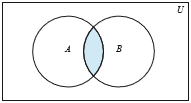
\includegraphics[scale=2.5]{chapter/imagens/32}
	\caption{Diagrama de Venn da intersecção de $A$ e $B$.}
	\label{fig32}
\end{figure}

\begin{exmp}
\label{exem316}
A intersecção dos conjuntos $\{1,3,5\}$ e $\{1,2,3\}$ é o conjunto $\{1,3\}$;
isto é $\{1,3,5\} \cap \{1,2,3\} = \{1,3\}$.
\end{exmp}

\begin{defn}
\label{def312}
Dois conjuntos são chamados de \emph{disjuntos} se a sua interseção é o conjunto
vazio (ou é nula).
\end{defn}

\begin{exmp}
\label{exem317}
Seja $A = \{1,3,5,7,9\}$ e $B = \{2,4,6,8,10\}$. Como $A \cap B = \emptyset$.
$A$ e $B$ são disjuntos.
\end{exmp}

Geralmente estamos interessados em encontrar a cardinalidade da união de dois
conjuntos finitos. Note que $|A| + |B|$ conta cada elemento em $A$ mas não em
$B$ ou em $B$ mas não em $A$ exactamente uma vez, e cada elemento que está em
ambos $A$ e $B$ é contado duas vezes. Assim, se o número de elementos que estão
ao mesmo tempo em $A$ e $B$ é subtraído de $|A|+|B|$, elementos em $A \cap B$
serão contados apenas uma vez. Dessa forma,
\begin{center}
$|A \cup B| = |A|+|B| - |A \cap B|$.
\end{center}

A generalização desse resultado para uniões de um número arbitrário de conjuntos
é chamado de \textbf{princípo de inclusão-exclusão}. Este princípio é
uma técnica importante utilizada em numeração.

Existem outras formas importantes de combinar dois conjuntos.

\begin{defn}
\label{def313}
Sejam $A$ e $B$ dois conjuntos. A \emph{diferença} entre $A$ e $B$, denotada por
$A - B$, é o conjunto que contém os elementos que existem em $A$ mas não existem
em $B$. A diferença entre $A$ e $B$ é também chamada de \emph{complemento} de
$B$ com respeito a $A$.
\end{defn}

\begin{description}
\item[Nota:] A diferença entre os conjuntos $A$ e $B$ é por vezes denotada por
$A\setminus B$.
\end{description}

Um elmento $x$ pertence a diferença entre $A$ e $B$ se e somente se $x \in A$ e
$x \notin B$. Isto nos diz que,
\begin{center}
$A - B = \{x \mid x \in A \land x \notin B\}$.
\end{center}

O diagrama de Venn apresentado na figura \ref{fig33} representa a diferença
entre os conjuntos $A$ e $B$.

\begin{figure}[H]
	\centering
	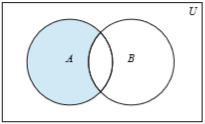
\includegraphics[scale=2]{chapter/imagens/33}
	\caption{Diagrama de Venn da diferença de $A$ e $B$.}
	\label{fig33}
\end{figure}

\begin{exmp}
\label{exem318}
A diferença entre $\{1,3,5\}$ e $\{1,2,3\}$ é o conjunto $\{5\}$; isto é,
$\{1,3,5\}-\{1,2,3\} = \{5\}$. Isto é diferente da diferença entre $\{1,2,3\}$ e
$\{1,3,5\}$, que é o conjunto $\{2\}$.
\end{exmp}

\begin{defn}
\label{def314}
Seja $U$ o conjunto universo. O complemento do conjunto $A$, denotado por
$\overline{A}$, é o complemento de $A$ com respeito a $U$. Assim, o complemento
do conjunto $A$ é $U - A$.
\end{defn}

Um elemento pertence a $\overline{A}$ se e somente se $x \notin A$. Isto nos diz
que,
\begin{center}
$\overline{A} = \{x \in U \mid x \notin A\}$.
\end{center}

Na figura \ref{fig34} a área sombreada fora do círculo que representa $A$ é a
área que representa $\overline{A}$.

\begin{figure}[H]
	\centering
	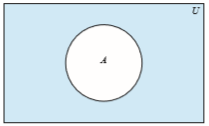
\includegraphics[scale=2]{chapter/imagens/34}
	\caption{Diagrama de Venn para o complemento de $A$.}
	\label{fig34}
\end{figure}


\begin{exmp}
\label{exem319}
Seja $A = \{a,e,i,o,u\}$, onde o conjunto-universo é o conjunto de todas as
letras do alfabeto, então $\overline{A} = \{b,c,d,f,g,h,j,\ldots,x,y,z\}$.
\end{exmp}

\begin{exmp}
\label{exem320}
Seja $A$ o conjunto dos números positivos inteiros maiores que 10 (onde o
conjunto universal é o conjunto de todos os positivos inteiros), então
$\overline{A} = \{1,2,3,4,5,6,7,8,9,10\}$.
\end{exmp}

\subsection*{\underline{Identidade de Conjuntos}}

A tabela \ref{tab:31} lista as identidades mais importantes dos conjuntos.
Iremos demonstrar algumas destas identidades utilizando três mêtodos diferentes.
Estes métodos são apresentados para ilustrar que geralmente existem diferentes
abordagens na resolução de um problema. As demonstrações das restantes
identidades serão deixadas como exercícios. Deverá notar também a similaridade
entre as identidades de conjuntos com as equivalências lógicas apresentadas no
capítulo \ref{cap:logicaformal}. Na verdade, as identidades de conjuntos
apresentadas podem demonstradas directamente das equivalências lógicas
correspondentes. Além disso, ambos são casos especiais de identidades da álgebra
de Boole.

\begin{table}[H]
	\centering
	\begin{tabular}{|l|l|}%
	\toprule
	\textbf{Identidade} & \textbf{Nome}\\
	\midrule
	$A \cap U = A$ &	Leis da Identidade\\
	$A \cup \emptyset = A$ &	\\
	\midrule
	$A \cup U = U$ &	Leis da Dominação\\
	$A \cap \emptyset = \emptyset$ &\\
	\midrule
	$A \cup A = A$ &	Leis da Idempotência\\
	$A \cap A = A$ &	\\
	\midrule
	$\overline{(\overline{A})} = A$ & Lei da Complementação\\
	\midrule
	$A \cup B = B \cup A$ & Leis Comutativas\\
	$A \cap B = B \cap A$ &\\
	\midrule
	$A \cup (B \cup C) = (A \cup B) \cup C$ & Leis Associativas\\
	$A \cap (B \cap C) = (A \cap B) \cap C$ &\\
	\midrule
	$A \cup (B \cap C) = (A \cup B) \cap (A \cup C)$ & Leis Distributivas
	\\
	$A \cap (B \cup C) = (A \cap B) \cup (A \cap C)$ & \\
	\midrule
	$\overline{A \cap B} = \overline{A} \cup \overline{B}$ & Leis de De Morgan\\
	$\overline{A \cup B} = \overline{A} \cap \overline{B}$ &\\
	\midrule
	$A \cup (A \cap B) = A$ & Leis da Absorção\\
	$A \cap (A \cup B) = A$&\\
	\midrule
	$A \cup \overline{A} = U$ & Leis do Complemento\\
	$A \cap \overline{A} = \emptyset$ &	\\
	\bottomrule%
	\end{tabular}%
	\caption{Idnetidades de conjuntos.}
	\label{tab:31}
\end{table}

Uma forma de demonstrar que dois conjuntos são iguais é por demonstrar que um é
subconjunto do outro e vice-versa. Lembre-se que para mostrar que um conjunto é
subconjunto de um outro conjunto, podemos mostrar que se um elemento pertence ao
primeiro conjunto então também deverá pertencer ao segundo conjunto. Geralmente
utilizamos uma demonostração directa para fazer isso. Iremos ilustrar este tipo
de demonstração por estabelecer a primeira lei de De Morgan.

\begin{exmp}
\label{exem321}
Demonstre que $\overline{A \cap B} = \overline{A} \cup \overline{B}$
\begin{description}
\item[Solução:] Iremos primeiramente demonstrar que os dois conjuntos
$\overline{A \cap B}$ e $\overline{A} \cup \overline{B}$ são iguais por provar
que cada um deles é subconjunto do outro. 

Primeiro, mostramos que $\overline{A \cap B} \subseteq \overline{A} \cup
\overline{B}$. Fazemos isto por provar que se $x$ está em $\overline{A \cap B}$,
então deverá também estar em $\overline{A} \cup \overline{B}$. Agora, suponha
que $x \in \overline{A \cap B}$. Pela definição do complemento, $x \notin A
\cap B$. Usando a definição de intersecção, vemos que a proposição $\lnot ((x
\in A) \land (x \in B))$ é verdadeira.

Ao aplicar a lei de De Morgan para as proposições, temos que $\lnot(x \in A)$ ou
$\lnot(x \in B)$. Utilizando a definição de negação das proposições, temos que
$x \notin A$ ou $x \notin B$. Utilizando a definição do complemento de um
conjunto, vemos que isto implica que $x \in \overline{A}$ ou $x \in
\overline{B}$. Consequentemente, pela definição da união, vemos que $x \in
\overline{A} \cup \overline{B}$. Temos agora demonstrado que $\overline{A
\cap B} \subseteq \overline{A} \cup \overline{B}$.

Agora, iremos mostrar que $\overline{A} \cup \overline{B} \subseteq
\overline{A \cap B}$. Fazemos isso por mostrar que se $x$ está em $\overline{A}
\cup \overline{B}$, então também deverá estar em $\overline{A \cap B}$. Suponha
agora que $x \in \overline{A} \cup \overline{B}$. Pela definição de união,
sabemos que $x \in \overline{A}$ ou $x \in \overline{B}$. Utilizando a definição
de complemento, vemos que $x \notin A$ ou $x \notin B$. Consequentemente, a
proposição $\lnot (x \in A) \lor \lnot (x \in B)$ é verdadeira.

Pela lei de De Morgan das proposições, concluímos que $\lnot ((x \in A) \lor
(x \in B))$ é verdadeira. Pela definição de intersecção, segue-se que $\lnot
(x \in A \cap B)$. Acabamos de utilizar a definição do complemento para concluir
que $x \in \overline{A \cap B}$. Isto mostra que $\overline{A} \cup
\overline{B} \subseteq \overline{A \cap B}$.

Como demonstramos que cada conjunto é subconjunto do outro, os dois conjuntos
são iguais e a identidade está provada.
\end{description}
\end{exmp}

Podemos agora mais sucintamente expressar este raciocínio no exemplo
\ref{exem321}, utilizando a notação de construção de domínios, tal como o
exemplo \ref{exem322} ilustra.

\begin{exmp}
\label{exem322}
Utilize a notação de construção de conjuntos e equivalências lógicas para
estabelecer a primeira lei de De Morgan $\overline{A \cap B} = \overline{A}
\cup \overline{B}$.
\begin{description}
\item[Solução:]Podemos provar esta identidade com os seguintes passos:

\begin{table}[H]
	\centering
	\begin{tabular}{rcll}%
	$\overline{A \cap B}$&$=$ & $\{x \mid x \notin A \cap B\}$ 			& \emph{pela
	definição do complemento}\\
	 					 &$=$ & $\{x \mid \lnot (x \in (A \cap B))\}$	& \emph{pela definição de
	 					 não pertença}\\
	 					 &$=$ & $\{x \mid \lnot (x \in A \land x \in B)\}$ & \emph{pela
	 					 definição de intersecção}\\
						 &$=$ & $\{x \mid \lnot(x \in A) \lor \lnot (x \in B)\}$ & \emph{pela
						 1a. lei de De Morgan para equivalências lógicas} \\
						 &$=$ & $\{x \mid x \notin A \lor x \notin B\}$ & \emph{pela definição de
						 não pertença}\\
						 &$=$ & $\{x \mid x \in \overline{A} \lor x \in \overline{B}\}$ &
						 \emph{pela definição do complemento}\\
						 &$=$ & $\{x \mid x \in \overline{A} \cup \overline{B}\}$ & \emph{pela
						 definição da união}\\
						 &$=$ & $\overline{A} \cup \overline{B}$ & \emph{pelo significado do
						 construtor de conjunto}			 
	\end{tabular}%
\end{table}
Note que para além das definições do complemento, união, pertença em conjuntos e
o construtor de conjuntos, esta demonstração utiliza a segunda lei de De Morgan
das equivalências lógicas.
\end{description}
\end{exmp}

\section{Funções}
\subsection*{\underline{Introdução}}

Em muitas instâncias atribuímos a cada elemento de um conjunto um outro elemento
particular de um segundo conjunto (que poderá ser o mesmo que o primeiro). Por
exemplo, suponha que a cada estudante na disciplina de Estruturas Discreta é
atribuído uma classificação do conjunto $\{10, 12, 13, 14, 17\}$.
Suponha também que estas notas são distribuídas a um grupo de alunos da seguinte
forma: 10 para o Aldo, 13 para a Carla, 12 para o Gabriel, 10 para a Rosa e 17
para o Samuel. Esta atribuição é ilustrada na figura \ref{fig35}.

\begin{figure}[H]
	\centering
 	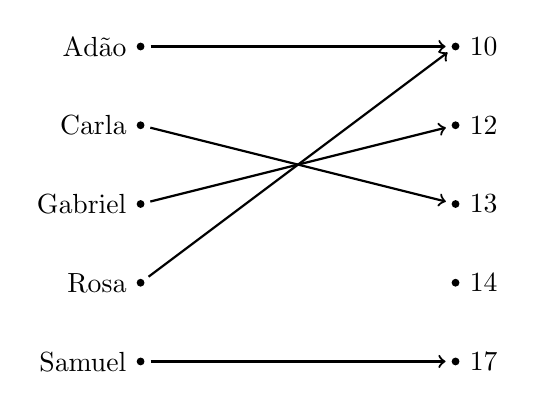
\begin{tikzpicture}[ele/.style={fill=black,circle,minimum width=.8pt,inner
 sep=1pt}] 
 
 	\node[ele,label=left:Adão] (a1) at (0,5) {};    
  	\node[ele,label=left:Carla] (a2) at (0,4) {};    
	\node[ele,label=left:Gabriel] (a3) at (0,3) {};
	\node[ele,label=left:Rosa] (a4) at (0,2) {};
	\node[ele,label=left:Samuel] (a5) at (0,1) {};
	\node[ele,,label=right:10] (b1) at (4,5) {};
	\node[ele,,label=right:12] (b2) at (4,4) {};
	\node[ele,,label=right:13] (b3) at (4,3) {};
	\node[ele,,label=right:14] (b4) at (4,2) {};
	\node[ele,,label=right:17] (b5) at (4,1) {};
	%\node[draw,fit= (a1) (a2) (a3) (a4),minimum width=2cm] {} ;
	%\node[draw,fit= (b1) (b2) (b3) (b4),minimum width=2cm] {} ;  
	\draw[->,thick,shorten <=2pt,shorten >=2pt] (a1) -- (b1);
	\draw[->,thick,shorten <=2pt,shorten >=2] (a2) -- (b3);
	\draw[->,thick,shorten <=2pt,shorten >=2] (a3) -- (b2);
	\draw[->,thick,shorten <=2pt,shorten >=2] (a4) -- (b1);
 	\draw[->,thick,shorten <=2pt,shorten >=2] (a5) -- (b5);
 	\end{tikzpicture}
 	\caption{Atribuição de notas na disciplina de Estrutura Discretas.}
	\label{fig35}
\end{figure}

Esta atribuição é um exemplo de uma função. O conceito de função é extremamente
importante em matemática e ciência da computação. Por exemplo, em
matemática discreta, funções são utilizadas  na definição destas estruturas
discretas como sequências. Funções também são também utilizadas para representar
quanto tempo um computador leva para resolver um problema de um determinado
tamanho. Muitos programas de computadores e subrotinas de programação, são
desenhadas para calcular valores de funções. Funções recursivas, que são
funções definidas em termos de sí próprias, são utilizadas extensivamente em
ciência da computação.

\begin{defn}
\label{def315}
Sejam $A$ e $B$ dois conjuntos não-vazios. A \emph{função} $f$ de $A$ para $B$ é
uma atribuição de exactamente um elemento de $B$ a cada elemento de $A$.
Escrevemos $f(a) = b$ se $b$ é um único elemento de $B$ atribuído pela função
$f$ ao elemento $a$ de $A$. Se $f$ é uma função de $A$ para $B$, escrevemos
$f:A \to B$.
\end{defn}

\begin{description}
\item[Nota:]Funções são por vezes chamadas \textbf{mapeamentos} ou
\textbf{transformações}.
\end{description}

As funções são especificadas de várias formas. Por vezes nós apresentamos as
atribuições explicitamente, como na figura \ref{fig35}. Geralmente utilizamos
uma fórmula, como $f(x)=x+1$, para definir uma função. Noutras ocasiões
utilizamos um programa de computador para especificar uma função.

A função $f:A \to B$ pode ser também definida em termos de uma relação de $A$
para $B$. Uma relação de $A$ para $B$ é apenas um subconjunto de $A \times B$. A
relação de $A$ para $B$ que contém um, e apenas um, par ordenado $(a,b)$ para
cada elemento $a \in A$, define a função $f$ de $A$ para $B$. Esta função é
definida pela atribuição de $f(a)=b$, onde $(a,b)$ é o único par ordenado na
relação que possui $a$ como o seu primeiro elemento.

\begin{defn}
\label{def316}
Se $f$ é uma função de $A$ para $B$, dizemos que $A$ é o \emph{domínio} de $f$ e
$B$ é o co-domínio de $f$. Se $f(a)=b$, dizemos que $b$ é a \emph{imagem} de $a$
e $a$ é a pré-imagem de $b$. O \emph{alcance}, ou \emph{imagem}, de $f$ é o
conjunto de todas as imagens dos elementos de $A$. Também, se $f$ é uma função
de $A$ para $B$, dizemos que $f$ \emph{mapeia} $A$ em $B$.
\end{defn}

A figura \ref{fig36} representa a função $f$ de $A$ para $B$.

\begin{figure}[H]
	\centering
	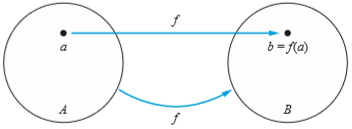
\includegraphics[scale=2]{chapter/imagens/36}
	\caption{Função $f$ que mapeia $A$ em $B$.}
	\label{fig36}
\end{figure}

Quando definimos uma função nós especificamos o seu domínio, co-domínio, e o
mapeamento dos elementos do domínio para os elementos no co-domínio. Duas
funções são \texbf{iguais} quando elas possuem o mesmo domínio, o mesmo
co-domínio, e mapeam cada elemento do domínio comum para os mesmos elementos do
co-domínio comum. Note que se mudarmos quer seja o domínio ou o co-domínio da
função, obteremos uma função diferente. Se mudarmos o mapeamento dos elementos,
obteremos também uma função diferente.

Os exemplos a seguir são exemplos de funções. Em cada exemplo, descrevemos o
domínio, o co-domínio, a imagem da função e a atribuição de valores para os
elementos do domínio.

\begin{exmp}
\label{exem323}
Seja $R$ a relação com os pares ordenados (André, 22), (Brenda, 24), (Carla,
21), (Doriel, 22), (Edna, 24) e (Felicia, 22). Cada um desses pares consiste no
nome de um estudante e a sua idade. Especifique uma função determinada por esta
relação?
\begin{description}
\item[Solução:]Se $f$ é a função especificada por $R$, então $f$(André) = 22,
$f$(Brenda) = 24, $f$(Carla) = 21, $f$(Doriel) = 22, $f$(Edna) = 24 e
$f$(Felicia) = 22. Aqui, $f(x)$ é a idade de $x$, onde $x$ é um estudante. Para
o domínio, temos o conjunto \{André, Brenda, Carla, Doriel, Edna, Felícia\}.
Precisamos também especificar o co-domínio, que deverá conter todas as idades
possíveis dos estudantes. Como é muito provável que os estudantes tenham todos
menos de 100 anos de idade, podemos indicar o conjunto dos números positivos
inteiros como o co-domínio. Note que poderíamos ter escolhido um co-domínio
diferente, como o conjunto dos inteiros positivos ou o conjunto dos inteiros
positivos entre 10 e 90, mas isto mudaria a função. Usar este co-domínio daria
também a possibilidade de extender a função por adicionar nomes e idades de mais
estudantes depois. A imagem da função especificada é o conjunto das diferentes
idades dos estudantes, que é o conjunto \{21,22,24\}.
\end{description}
\end{exmp}

\begin{exmp}
\label{exem324}
Seja $f$ a função que atribui os dois últimos bits de uma cadeia de bits de
tamanho 2 ou superior, a tal cadeia. Por exemplo $f(11010) = 10$. Assim, o
domínio de $f$ é o conjunto de todas as cadeias de bits de tamanho superior a 2,
e o co-domínio e a imagem são o conjunto $\{00,01,10,11\}$.
\end{exmp}

\begin{exmp}
\label{exem325}
Seja $f: \mathbf{Z} \to \mathbf{Z}$ que atribui o quadrado de um número inteiro
a este número. Então, $f(x) = x^2$, onde o domínio de $f$ é o conjuntos de
todos os números inteiros, o co-domínio de $f$ é o conjunto dos números
inteiros, e a imagem de $f$ é o conjunto de todos inteiros que são quadrados
perfeitos, nomeadamente, $\{0,1,4,9,\ldots\}$.
\end{exmp}

\begin{exmp}
\label{exem326}
O domínio e o co-domínio de funções geralmente são especificados em linguagens
de programação. Por exemplo, a seguinte expressão em Java
\begin{center}
\texttt{int piso (double num)\{\ldots\}}
\end{center}
nos diz que o domínio da função \texttt{piso} é o conjunto dos números
reais (representado pelo tipo de dados \texttt{double}) e o seu co-domínio é o
conjunto dos números inteiros.
\end{exmp}


\begin{defn}
\label{def317}
Sejam $f_1$ e $f_2$ funções de $A$ para $\mathbf{R}$. Então $f_1 + f_2$ e
$f_1f_2$ são também funções de $A$ para $\mathbf{R}$ definidas para todo $x \in
A$ por

\begin{center}
$(f_1+f_2)(x) = f_1(x) + f_2(x)$,\\
$(f_1f_2)(x) = f_1(x)f_2(x)$.
\end{center}

Note que as funções $f_1+f_2$ e $f_1f_2$ foram definidas pela especificação dos
seus valores em $x$ em termos dos valores de $f_1$ e $f_2$ em $x$.
\end{defn}

\begin{exemp}
\label{exem327}
Sejam $f_1$ e $f_2$ duas funções de $\mathbf{R}$ em $\mathbf{R}$ tal que
$f_1(x) = x^2$ e $f_2(x) = x - x^2$. Quais são os valores das funções $f_1 +
f_2$ e $f_1f_2$?
\begin{description}
\item[Solução:] Da definição da soma e produto de funções, temos que
\begin{center}
$(f_1 + f_2)(x) = f_1(x) + f_2(x) = x^2 + (x - x^2) = x$,
\end{center}
e
\begin{center}
$(f_1f_2)(x)=x^2(x-x^2) = x^3-x^4$.
\end{center}
\end{description}
\end{exemp}
Quando $f$ é uma função de $A$ para $B$, a imagem de um subconjunto de $A$
também pode ser definida.


\begin{defn}
\label{def318}
Seja $f$ uma função de $A$ para  $B$ e seja $S$ um subconjunto de $A$. A
\emph{imagem} de $S$ sobre a função $f$ é o subconjunto de $B$ que consiste nas
imagens dos elementos de $S$. Denotamos a imagem de $S$ por $f(S)$, tal que
\begin{center}
$f(S) = \{t \mid \exists s \in S (t = f(s))\}$.
\end{center}
Também podemos utilizar a notação curta $\{f(s) \mid s \in S\}$ para denotar
este conjunto
\begin{description}
\item[Nota:]A notação $f(S)$ para a imagem do conjunto $S$ sobre a função $f$ é
potencialmente ambígua. Aqui, $f(S)$ denota um conjunto e não o valor da função
$f$ no conjunto $S$.
\end{description}
\end{defn}

\begin{exmp}
\label{exem328}
Seja $A = \{a,b,c,d,e\}$ e $B=\{1,2,3,4\}$ com $f(a)=2$, $f(b)=1$, $f(c)=4$,
$f(d)=1$ e $f(e)=1$. A imagem do subconjunto $S=\{b,c,d\}$ é o conjunto
$f(S)=\{1,4\}$.
\end{exmp}


\subsection*{\underline{Funções injectivas e sobrejectivas}}

Algumas funções nunca atribuiem o mesmo valor para dois elementos diferentes do
domínio. Estas funções são chamadas de \texbf{injectivas}.

\begin{defn}
\label{def320}
A função $f$ é chamada de uma \emph{injunção}, se e somente se $f(a) = f(b)$
implica que $a=b$ para todo $a$ e $b$ no domínimo de $f$. A função é chamada de
\emph{injectiva} se for uma injunção.
\end{defn}

Note que um função $f$ é injectiva se e somente se $f(a) \neq f(b)$ sempre que
$a \neq b$. Esta forma de expressar que $f$ é uma injunção é obtida por obter a
contrapositiva da implicação na definição.

\begin{description}
\item[Nota:]Podemos expressar que $f$ é uma injunção utilizando quantificadores
como $\forall a\forall b (f(a)=f(b) \to a = b)$ ou equivalentemente $\forall
a\forall b(a \neq b \to f(a) \neq f(b))$, onde o universo em discurso é o
domínio da função.
\end{description}

Ilustraremos este conceito com alguns exemplos de funções que são injectivas e
outras que não são.

\begin{exmp}
\label{exem329}
Determine se a função $f$ de $\{a,b,c,d\}$ para $\{1,2,3,4,5\}$ com $f(a)=4$,
$f(b)=5$, $f(c)=1$ e $f(d)=3$ é injectiva.
\begin{description}
\item[Solução:]A função $f$ é injecetiva porque $f$ obtém valores diferentes nos
quatro elementos do seu domínio. Isto é ilustrado na figura \ref{fig37}.
\end{description}
\end{exmp}

 \begin{figure}[H]
	\centering
 	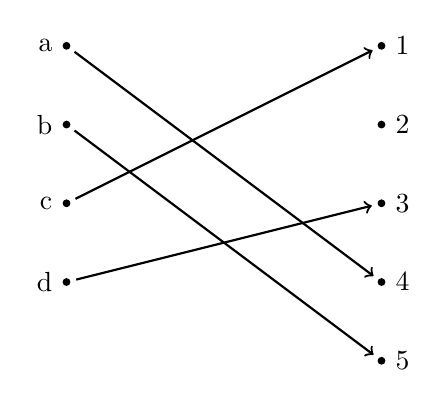
\begin{tikzpicture}[ele/.style={fill=black,circle,minimum width=.8pt,inner
 sep=1pt}] 
 
 	\node[ele,label=left:a] (a1) at (0,5) {};    
  	\node[ele,label=left:b] (a2) at (0,4) {};    
	\node[ele,label=left:c] (a3) at (0,3) {};
	\node[ele,label=left:d] (a4) at (0,2) {};
	\node[ele,,label=right:1] (b1) at (4,5) {};
	\node[ele,,label=right:2] (b2) at (4,4) {};
	\node[ele,,label=right:3] (b3) at (4,3) {};
	\node[ele,,label=right:4] (b4) at (4,2) {};
	\node[ele,,label=right:5] (b5) at (4,1) {};
	%\node[draw,fit= (a1) (a2) (a3) (a4),minimum width=2cm] {} ;
	%\node[draw,fit= (b1) (b2) (b3) (b4),minimum width=2cm] {} ;  
	\draw[->,thick,shorten <=2pt,shorten >=2pt] (a1) -- (b4);
	\draw[->,thick,shorten <=2pt,shorten >=2] (a2) -- (b5);
	\draw[->,thick,shorten <=2pt,shorten >=2] (a3) -- (b1);
	\draw[->,thick,shorten <=2pt,shorten >=2] (a4) -- (b3);
 	\end{tikzpicture}
 	\caption{Uma função injectiva.}
	\label{fig37}
\end{figure}

\begin{exmp}
\label{exem330}
Determine se a função $f(x)=x^2$ do conjunto dos números inteiros para o
conjunto dos números inteiros é injectiva.

\begin{description}
\item[Solução:]A função $f(x)=x^2$ não é injectiva porque, por exemplo,
$f(1)=f(-1)=1$, mas no entanto $1 \neq -1$.
Note que a função $f(x)=x^2$ com os seus domínios restrictos de \textbf{Z}$^+$ é
injectiva. (Tecnicamente, quando restringimos o domínio de uma função, obtemos
uma nova função cujos valores coincidem com os mesmo valores da função original
para os elementos do domínio restricto. A função restricta não é definida para
os elementos do domínio original fora do domínio restricto.)
\end{description}
\end{exmp}

\begin{exmp}
\label{exem331}
Determine se a função $f(x)=x+1$ do conjunto dos números reais para o mesmo
conjunto é injectiva.
\begin{description}
\item[Solução:]A função $f(x)=x+1$ é uma função injectiva. Para demonstrar isto,
note que $x+1 \neq y+1$ quando $x \neq y$.
\end{description}
\end{exmp}

\begin{defn}
\label{def321}
Uma função $f$ cujo domínio e co-domínio são subconjuntos do conjuntos dos
números reais é chamada de \emph{crescente} se $f(x) \leq f(y)$, e
\emph{estritamente crescente} se $f(x) < f(y)$, quando $x<y$ e $x$ e $y$ estão
no domínio de $f$.
Similarmente, $f$ é chamada de \emph{decrescente} se $f(x) \geq f(y)$, e
\emph{estritamente decrescente} se $f(x) > f(y)$, sempre que $x<y$ e $x$ e $y$
estão no domínio de $f$. (A palavra \emph{estritamente} nesta definição indica
que desigualdade.)
\end{defn}

\begin{description}
\item[Nota:]Uma função $f$ é crescente se $\forall x\forall y(x<y \to f(x) \leq
f(y))$, estritamente crescente se $\forall x\forall y(x<y \to f(x) < f(y))$,
decrescente se $\forall x\forall y(x<y \to f(x) \geq f(y))$ e estritamente
decrescente se $\forall x\forall y(x<y \to f(x) > f(y))$, onde o universo de
discurso é o domínio de $f$.
\end{description}

\begin{defn}
\label{def322}
A função $f$ de $A$ para $B$ é chamada de \emph{sobrejectiva}, se e somente se
para cada elemento $b \in B$ existe um elemento $a \in A$ com $f(a)=b$.

\begin{description}
\item[Nota:]A função $f$ é sobrejectiva se $\forall y\exists x(f(x)=y)$, onde o
domínio para $x$ é o domínio da função e o domínio para $y$ é o co-domínio da
função.
\end{description}
\end{defn}

\section{Matrizes}
\section{Sequências}